% Created 2019-10-02 Wed 16:57
% Intended LaTeX compiler: pdflatex
\documentclass[presentation]{beamer}
\usepackage[utf8]{inputenc}
\usepackage[T1]{fontenc}
\usepackage{graphicx}
\usepackage{grffile}
\usepackage{longtable}
\usepackage{wrapfig}
\usepackage{rotating}
\usepackage[normalem]{ulem}
\usepackage{amsmath}
\usepackage{textcomp}
\usepackage{amssymb}
\usepackage{capt-of}
\usepackage{hyperref}
\institute{Universidad Nacional Autónoma de México}
\usetheme{metropolis}
\usecolortheme{}
\usefonttheme{}
\useinnertheme{}
\useoutertheme{}
\author{Adrián Antonio Rodríguez Pié}
\date{2 de octubre de 1968}
\title{Implementación de redes neuronales convolucionales para el meta-análisis de acoplamientos moleculares de complejos proteína-ligando}
\AtBeginSection{\frame{\sectionpage}}
\metroset{block=fill}
\hypersetup{
 pdfauthor={Adrián Antonio Rodríguez Pié},
 pdftitle={Implementación de redes neuronales convolucionales para el meta-análisis de acoplamientos moleculares de complejos proteína-ligando},
 pdfkeywords={},
 pdfsubject={},
 pdfcreator={Emacs 26.3 (Org mode 9.1.9)},
 pdflang={English}}
\begin{document}

\maketitle
\begin{frame}{Outline}
\tableofcontents
\end{frame}



\section{Sobre inteligencia artificial}
\label{sec:org92ad795}
\begin{frame}[label={sec:orge7ef6c1}]{La prueba de Turing}
\begin{center}
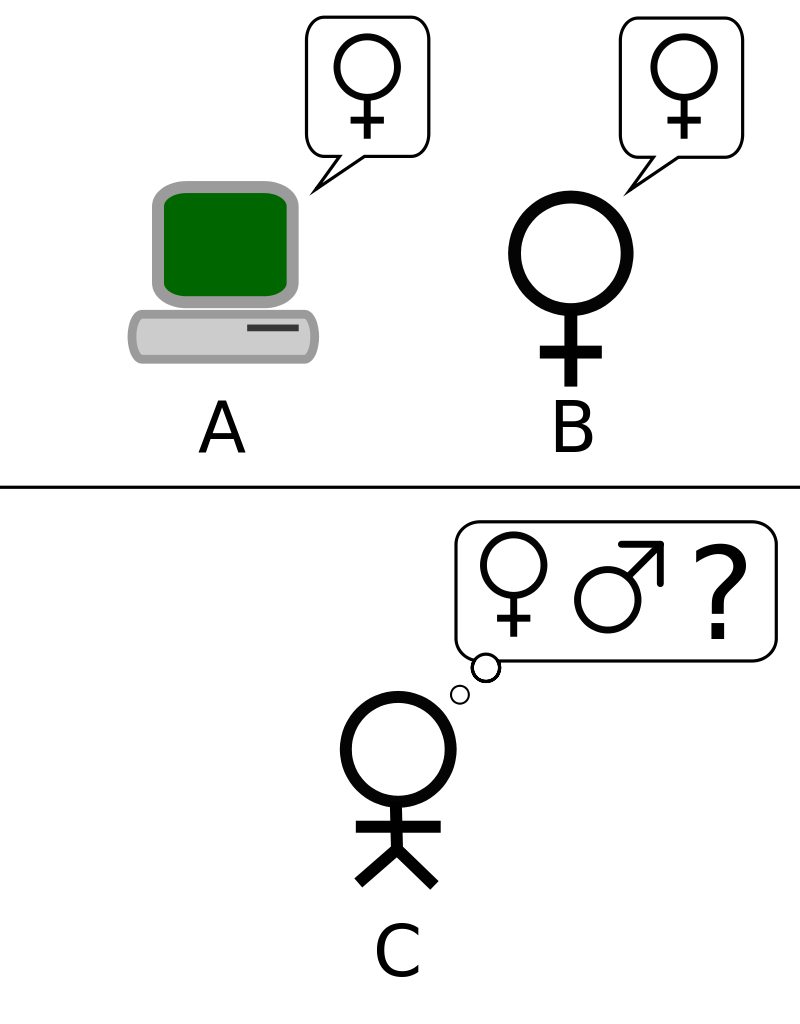
\includegraphics[width=170px]{images/turing-test.png}
\end{center}
\end{frame}
\begin{frame}[label={sec:orgd4b6aa2}]{IA y agentes}
\begin{block}{Inteligencia artrificial}
\alert{\alert{Agentes racionales}} que, mediante \alert{\alert{sensores}} pueden
percibir su \alert{\alert{entorno}} y actuar sobre él a partir de un
sistema de decisión.
\pause
\end{block}
\begin{block}{Agentes}
Máquina compuesta por un conjunto finito de estados, cuyas
transiciones están dadas por reglas de inferencias.
\end{block}
\end{frame}
\begin{frame}[label={sec:org9e02f30}]{Tipos de aprendizaje}
\begin{itemize}
\item Supervisado vs no supervisado
\item Agentes pasivos vs pasivos
\item Ayuda del profesor
\item Entrenamiento lineal vs por lote
\end{itemize}
\end{frame}
\section{Regunda chgapter o algo así?}
\label{sec:org4169104}
\begin{frame}[label={sec:org0934856}]{Segundoeeeee}
\begin{block}{This should be a block}
I hope it works correctly
\end{block}
\end{frame}
\end{document}
